\documentclass[runningheads,a4paper]{llncs}

\usepackage[english]{babel}
\usepackage{ifpdf}
\usepackage{hyperref}
\usepackage{cite}
%\usepackage[cmex10]{amsmath}

\usepackage{array}
\usepackage{mdwmath}
\usepackage{mdwtab}

%\usepackage{caption}
%\usepackage{subcaption}
%\usepackage{subfig} 


\usepackage{fixltx2e}
\usepackage{stfloats}
\usepackage{float}
\usepackage{graphicx} % Required for the inclusion of images
\usepackage{amsmath} % Required for some math elements 
%\usepackage{caption}

\usepackage{url}
\usepackage{algorithmic}
\usepackage{enumitem}
\usepackage{subfigure}
\usepackage{comment}
\makeatletter

\usepackage{color}
\usepackage{amssymb}


\usepackage{fancyvrb}
\newcommand{\ygg@basicalert}[2]{\fbox{\bfseries\sffamily\scriptsize#1}{\sf\small$\blacktriangleright$\textit{#2}$\blacktriangleleft$}}
\newcommand{\annote}[2]{\ygg@basicalert{\textsc{#1}}{\textcolor{red}{#2}}}

%\newcommand{\annote}[2]{\ygg@basicalert{\textsc{#1}}{\textcolor{red}{#2}}}
\newcommand{\mohamed}[1]{\annote{Mohamed}{#1}}
\newcommand{\todomohamed}[1]{\annote{TODO-Mohamed}{#1}}

\newcommand{\katrina}[1]{\annote{Katerina}{#1}}
\newcommand{\todokatrina}[1]{\annote{TODO-Katerina}{#1}}
%
\newcommand{\heiko}[1]{\annote{Heiko}{#1}}
\newcommand{\todoheiko}[1]{\annote{TODO-Heiko}{#1}}

\newcommand{\pramod}[1]{\annote{Pramod}{#1}}
\newcommand{\todopramod}[1]{\annote{TODO-Pramod}{#1}}

\newcommand{\obinna}[1]{\annote{Obinna}{#1}}
\newcommand{\todoobinna}[1]{\annote{TODO-Obinna}{#1}}
%
\newcommand{\gabriel}[1]{\annote{Gabriel}{#1}}
\newcommand{\todogabriel}[1]{\annote{TODO-Gabriel}{#1}}

\newcommand{\bryan}[1]{\annote{Bryan}{#1}}
\newcommand{\todobryan}[1]{\annote{TODO-Bryan}{#1}}

\newcommand{\all}[1]{\annote{all}{#1}}
\newcommand{\todoall}[1]{\annote{TODO-All}{#1}}

\usepackage{listings}
   
\newcommand{\keywords}[1]{\par\addvspace\baselineskip
\noindent\keywordname\enspace\ignorespaces#1}
\makeatother

\begin{document}
\mainmatter  % start of an individual contribution

% first the title is needed
\title{rSLA: Monitoring SLAs in dynamic service environments}

% the name(s) of the author(s) follow(s) next
%
% NB: Chinese authors should write their first names(s) in front of
% their surnames. This ensures that the names appear correctly in
% the running heads and the author index.
%

\author{Heiko Ludwig\and Mohamed Mohamed\and Katerina Stamou\and\\ Nagapramod Mandagere\and
Bryan Langston\and Gabriel Alatorre\and\\ Hiroaki Nakamura\and
Obinna Anya\and Alexander Keller}
%
\authorrunning{H. Ludwig et al.}
% (feature abused for this document to repeat the title also on left hand pages)

% the affiliations are given next; don't give your e-mail address
% unless you accept that it will be published
\institute{IBM Research\\
Email:\{hludwig, mmohamed, stamou, pramod, bryanlan, galatorr, obanya, alexk\}@us.ibm.com\\
{hnakamur@jp.ibm.com}}

%
% NB: a more complex sample for affiliations and the mapping to the
% corresponding authors can be found in the file "llncs.dem"
% (search for the string "\mainmatter" where a contribution starts).
% "llncs.dem" accompanies the document class "llncs.cls".
%

%\toctitle{Lecture Notes in Computer Science}
%\tocauthor{Authors' Instructions}
\maketitle

\begin{abstract}
Today's application environments combine Cloud and on-premise infrastructure as well as platforms and services from different providers to enable the quick development and 
delivery of solutions to their intended users. For example, a Web or mobile application of an online merchant might be deployed on a cloud-based Platform-as-a-Service, use 
persistence services within the platform, run ID and login management through a third-party Web service, and be monitored by various in-house logistics systems. The ability to use 
Cloud platforms to stand up applications in a short time frame, the - now - wide availability of services, and the application of a continuous deployment model has led to a much 
more dynamic application environment, changing at high velocity.

Managing quality of service has become more important and also poses new challenges in this more complex and dynamic environment. The more external service vendors involved the 
less control an application owner has and must rely on the quality commitments of his or her vendors in the form of a Service Level Agreement (SLA). Adding to the complexity, 
services from different vendors expose different instrumentation and use different service management systems making it difficult to collect and aggregate performance data for 
service level objective evaluation. In addition, the increasing dynamism of application environments entails that SLA monitoring must be set up at the same speed of changes to the 
application environment.  

Current SLA management systems often lack the flexibility to deal with instrumentation of heterogeneous environments and the agility to set up a new SLA instantaneously. This 
paper proposes the rSLA service that is both flexible enough to instrument virtually any environment and agile enough to scale and update SLA management as needed. Given an SLA 
expressed using a formal SLA specification, rSLA sets up the monitoring infrastructure and starts monitoring compliance. Using rSLA the time of setting up SLA compliance monitoring 
of application environments involving infrastructure, platform, and application services can be significantly reduced and aligned with typical application.

\keywords{Service Level Agreement, Cloud Computing, PaaS, Monitoring, Reporting }
\end{abstract}


%Xlet abstraction, 
sla language  xlets, easy to use language, run it as a service, fast to deploy, solution for sla management and cheap the 

clarify why now: dealing with heterogeneity (wsla applications in application server) notion of service is much more vigor, micro services,  extensibility and customizability, the introduction of devops make infrastructure changes more often than code changes, code agility, 

cloud apps today are being solved by horizontal scaling, once we deploy latency intensive applications SLAs become a must. 

why now: we are running on shared everything infrastructures, the desire to use SLAs is greater








\section{Introduction}\label{sec:introduction}

rSLA is a domain specific language (DSL) for expressing and managing service level agreements (SLAs) in a cloud environment. rSLA is coded in Ruby \cite{ruby}, a dynamic language that enables rapid prototyping and application development. 

The rSLA DSL is described by an alphabet and by production rules that help to extend the language. The rSLA programming library provides a runtime engine for deploying and running an rSLA service in a cloud environment.

Although the scientific literature provides plentiful results on automated management of SLAs for distributed computing \cite{wsla, wsag}, cloud markets hesitate to adopt such solutions. Provisioning of cloud services is handled either manually or with software tools that do not embrace cloud service characteristics.

Cloud service management does not yet support automated and transparent solutions for the management of leased resources. Additionally, there is no established standard yet for the automatic expression and management of SLAs for cloud services.

rSLA provides a DSL library for the definition of rSLA objects and a runtime engine to create and process such objects. The DSL enables the automated generation of customized SLAs and the transparent management of cloud service compliance.

The rSLA is deployed on the IBM Bluemix platform \cite{bluemix} as a ruby web service using the sinatra gem\footnote{Sinatra, \url{http://www.sinatrarb.com/}}. A pilot version of the language is currently running for an IBM financial client. The monthly results from using the rSLA language to evaluate the service level compliance of resources leased by the client, showcase the rSLA DSL adequacy in managing cloud services.

How is the paper structured

-what is the problem that the language solves, motivation to solve this problem
-language structure, alphabet, production rules
-language runtime
-current testing, future testing 


\section{Problem definition/ Motivation}\label{problem}
\todoheiko{Introduction, Motivation, Abstract}\\
\todogabriel{Introduction, Motivation, Abstract}
Cloud service management has not yet integrated automated and transparent solutions for controlling the provisioning of resources. Cloud customers pay for applications, however they do not have tools to verify their applications' service level values. Similarly, cloud providers do not have tools to evaluate on-demand their service level compliance and to optimally control their resource distribution.

There is no established standard for the automated expression and management of SLAs for cloud services. The research community has proposed solutions for defining SLA context \cite{wsla, wsag} and for processing such information \cite{lisa, lessons} in a distributed computing environment. The cloud industry, however, has not adopted any methods for the automatic management and evaluation of service level values.

SLA terms enclose data values that are retrieved from monitoring. Monitoring in this context means the systematic observation of metric values that are used by one or more services. An SLA may include numerous such values, which in turn are processed for the evaluation of service level objectives (SLOs). In service level management, an SLO verifies if SLA conditions are violated or not. A cloud provider needs to control during service runtime the value levels of countless SLOs from multiple customers. Cloud markets do not yet provide such tools.

A scheduler is used to coordinate the execution of involved processes for the systematic control of service level values. A cloud scheduler executes tasks that define the monitoring of service metrics and that perform the evaluation of service values at defined points during a service runtime. In a cloud environment, a scheduler additionally takes into account the availability of cloud resources and their distribution among service customers. 
 
In service level management, there are functional and operational dependencies between involved entities. For example, a composite metric, as its name implies, represents the composition result from one or more base, as well as composite metric values. The values of composite metrics in an SLA are used for the definition of conditions and objectives on service levels. 

Hence, a schedule configuration for measuring base metric values, may impact the evaluation schedule for one or more composite metric values. Such dependencies raise research questions on how optimal scheduling configurations can apply in a cloud environment for service measurement and evaluation tasks.
 
Evaluation of service levels consists from multiple computing tasks. SLOs are evaluated in scheduled intervals to determine service level compliance. An evaluation process may define a set of SLO conditions.  Such conditions take the form of logical statements that are configured in the SLO definition. Logical statements may require to compare a set of composite values against one or more threshold values. 

rSLA provides an SLA programming library and a service runtime engine for creating and managing SLAs in a cloud environment. The language is not intended to be used only by engineers or ruby developers. An important goal of the rSLA design is to provide a high-level, easy to use and to extend tool that is suitable either for human or machine consumption.


IBM Bluemix is a cloud-based platform to build, run and manage applications. 


%\section{Related work}
\todoobinna{Related work}

\todokatrina{Related work}

The scientific literature has proposed solutions for the automated management of SLA services that run over web \cite{wsla} and/or distributed \cite{SNAP, wsag} environments. WS-Agreement \cite{wsag} inherits language characteristics of the WSLA specification and has been used in numerous grid or cloud research initiatives \cite{soi, lessons, butler}.



\section{Overview of the Approach}

The key objective of our SLA compliance monitoring system presented in this paper is fast deployment in an environment in which the subject of monitoring is evolving quickly and services expose a variety of measurement interfaces. This section provides an overview of our approach how to address those issues at the same time. The first subsection discusses the system model outlining how the rSLA service interacts with interfaces of a heterogeneous environment. The second part outlines the major elements of an SLA document's content.

\subsection{System Model}

Cost, availability and on-demand scaling have accelerated customer adoption of different application deployment models - On-Premise cloud, Private cloud, Public cloud or hybrid 
clouds, in addition to their traditional dedicated environments. Depending on the services that an application depends on, the choice of platform varies. A single application could potentially be reliant on multiple clouds for the set of 
services it consumes. From a customer/tenant perspective, monitoring service levels that their workloads are getting often becomes a complex task of aggregating information across 
multiple cloud providers, each using different proprietary monitoring and management stacks. Further aggravating the problem is the devops transition. Applications and consequently 
their bindings to services are seeing an increased rate of change. 

\begin{figure}[H]
\centering
 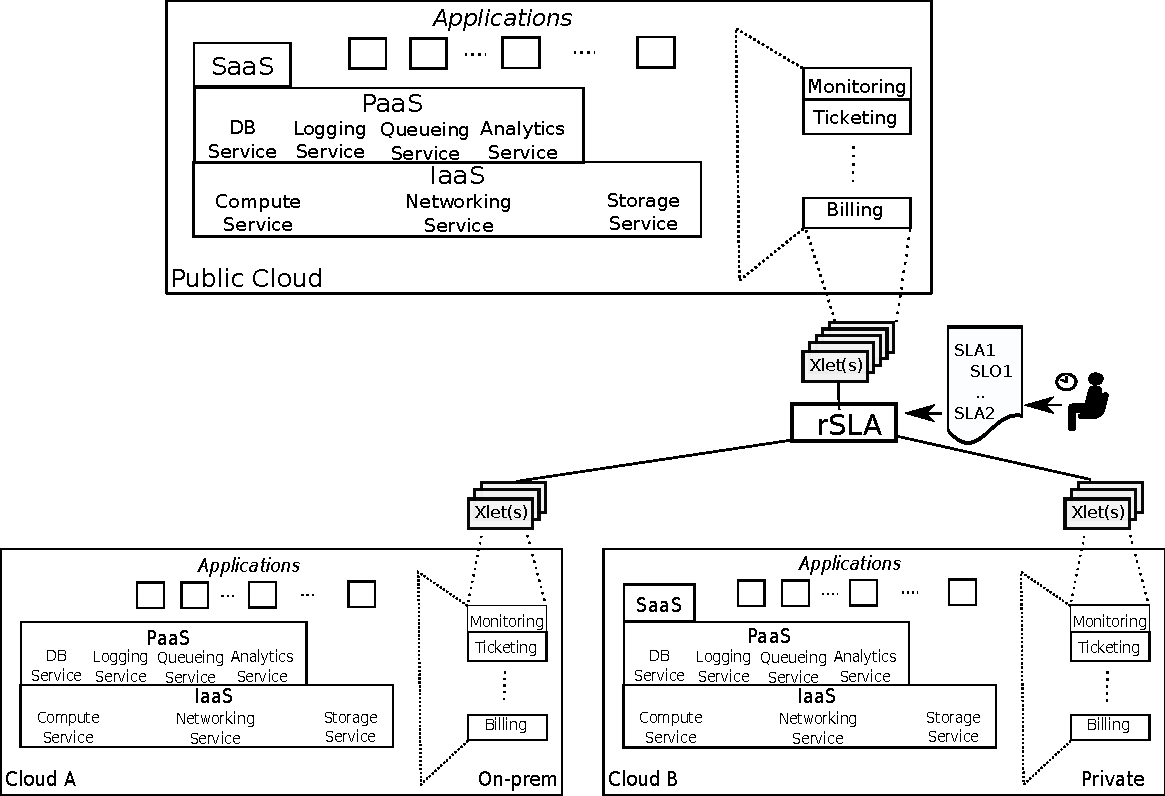
\includegraphics[width=8cm,height=8cm]{pics/systemModel.pdf} 
 \caption{rSLA System Overview}
 \label{fig:systemModel}
\end{figure}

Figure \ref{fig:systemModel} shows an overview of the proposed rSLA system model. The rSLA framework is made up three main components:
\begin{enumerate}
\item a language for administrators or service providers to express service level agreements; 
\item a set of  Xlets - lightweight, dynamically bound adapters; xlets abstract the heterogeneity of service management interfaces to rSLA, both for the reading of metrics as well as the acting on the result of SLA evaluation; and
\item a modular SLA evaluation service; this service interprets the rSLA document. It performs the reading of measurements through monitoring xlets as defined in the document, aggregates metrics, evaluated compliance and then notifies stakeholders.
\end{enumerate}

A formal language for SLAs is the key to both custom SLAs on a case-by-case basis and fast deployment of the SLA. The xlet approach provides the level of abstraction and indirection to intermediate between service interface heterogeneity and the need of the SLA evaluation service to read metrics in a homogenous way. 

The rSLA evaluation itself can be deployed in any 
of the cloud deployment models - On-Premise cloud, Private cloud, Public cloud or hybrid clouds. Further sections describe the language concepts, the execution model, and implementation. The case study discusses some xlets we wrote for a particular Cloud service.





\section{rSLA language}

Cloud SLA management can be costly. A provider needs to control resources that are used by multiple tenants. Every tenant agrees on service levels that can be different from those of other customers. To guarantee service level compliance, a provider monitors service level values and schedules measurement and evaluation operations for all active service level agreements. 

Such practices require instrumentation of monitoring, scheduling and data storage tools that can be tedious to deploy for someone unfamiliar with IT. In addition, such practices are performed systematically.  A semantic vocabulary is required to orchestrate their processing. 

The rSLA language can be deployed as a cloud service and provide all such service level management practices on-demand. On top, such deployment in a cloud environment is inexpensive because rSLA has minimal external tool dependencies. 

%alphabet, vocabulary, language structure, production rules 
%add reference to the rSLA spec
%conceptual model on how we think about metrics, services, SLOs, Xlets

\subsection{rSLA language conceptual model}
%notion of service, metric in the abstract
A service, in an rSLA runtime environment, is described by its provisioning compliance levels, which in turn are decomposed into multifarious service management elements. The rSLA language follows the semantic decomposition of the WSLA specification \cite{wsla}, where an SLA takes the form of a directed graph that has a single root vertex. The root node is connected to three vertices that denote primary branches of the hierarchical tree.

In an rSLA tree, the root vertex represents a single SLA object. Figure \ref{treegraph} illustrates programming objects of the rSLA language. Semantic connections between such objects compose an rSLA tree (Figure \ref{rslaobject}). Formalizing such tree as a directed graph helps with the structured management of either vertices or edges (Figure \ref{rslagraph}).

\begin{figure}
        \centering
        \begin{subfigure}{5cm}
                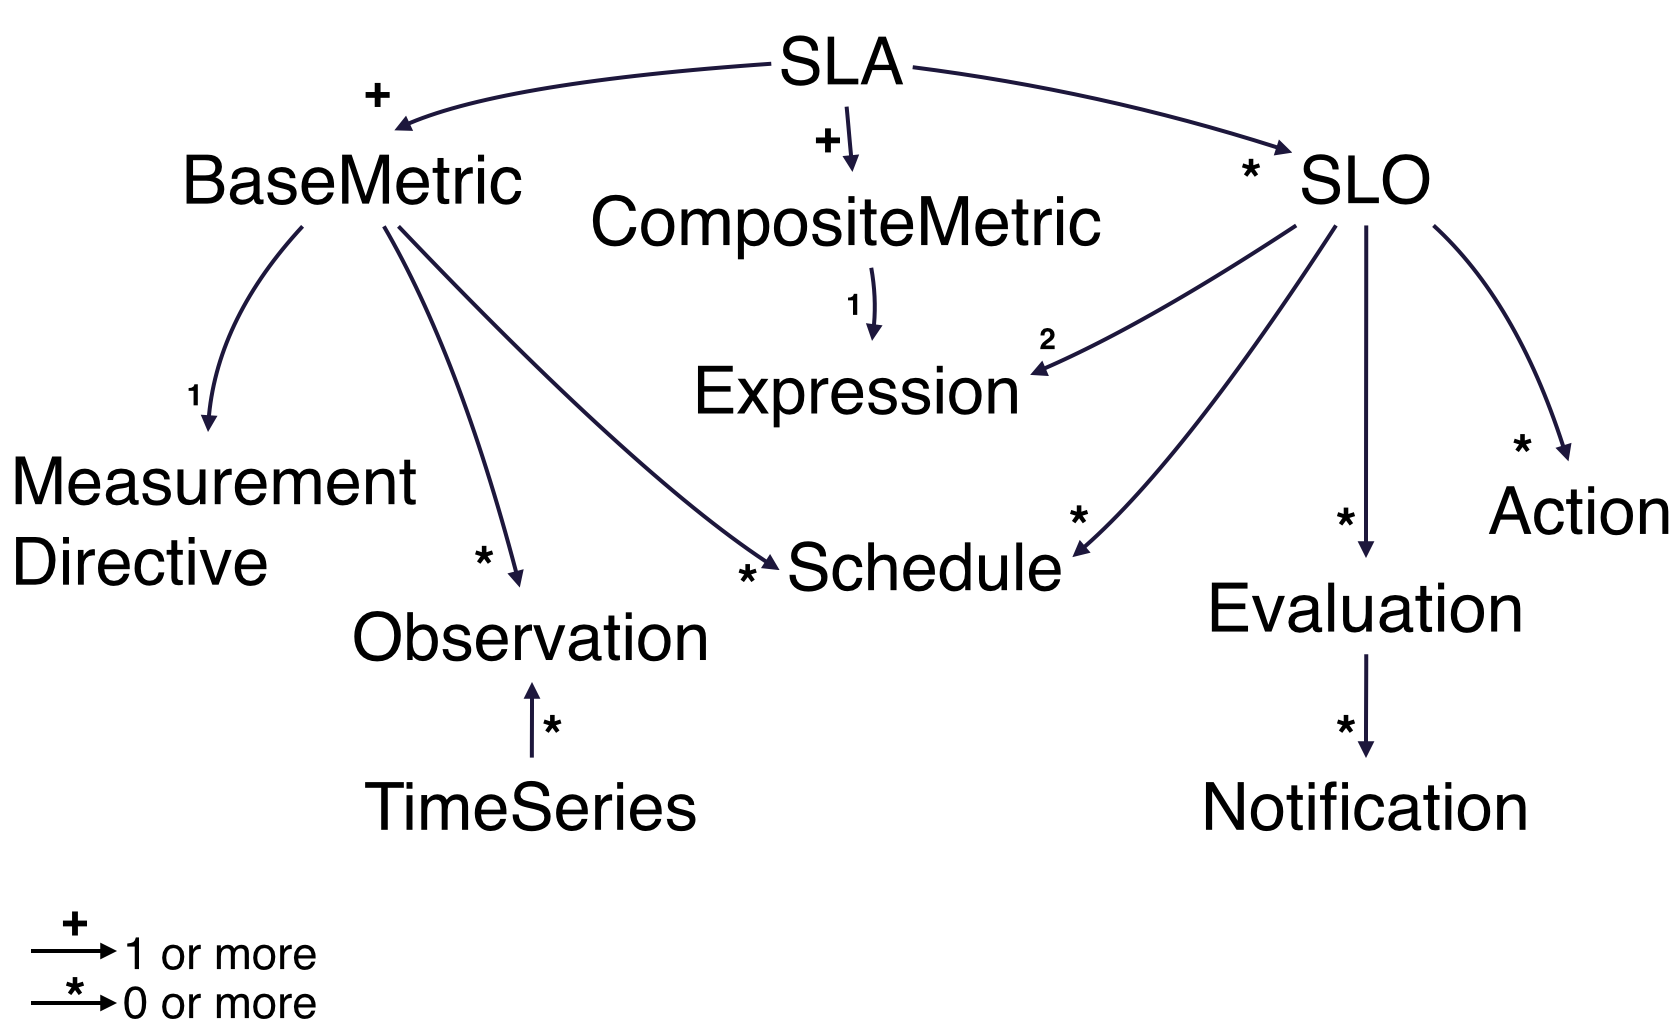
\includegraphics[height=3cm]{pics/rslaobject}
                \caption{rSLA object tree}
                \label{rslaobject}
        \end{subfigure}%
        \begin{subfigure}{5cm}
              %  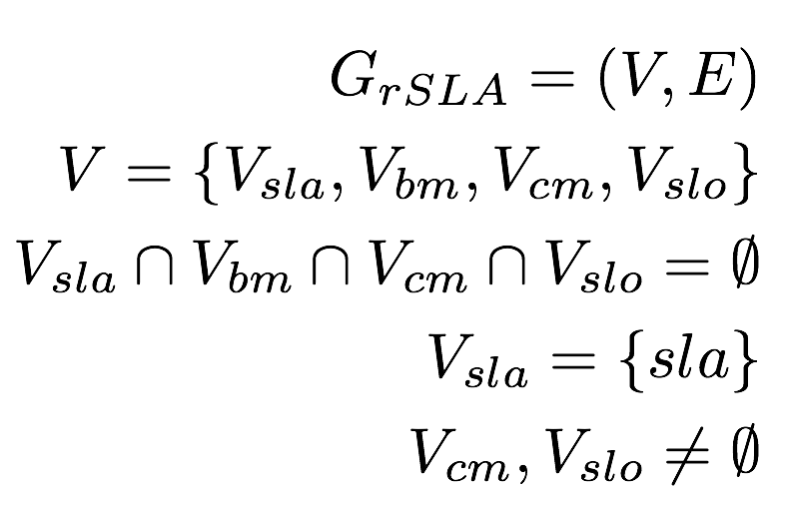
\includegraphics[height=3cm]{pics/rslagraph}
                \caption{rSLA vocabulary formalization}
                \label{rslagraph}
        \end{subfigure}
        \caption{rSLA vocabulary}\label{treegraph}
\end{figure}

Nodes that are close to the tree root in Figure \ref{rslaobject}, designate SLA branches like base, composite metrics and service level objectives. Edges between nodes are uni-directed to illustrate the rSLA tree hierarchy. The edge direction points to the nested element in the hierarchical relationship. 
Edges in Figure \ref{rslaobject} are labeled with +, * or number symbols to indicate that the multiplicity of nested objects. Hence, an SLA can be defined by sets of base, composite metric and SLO objects.

In an rSLA runtime environment, a base metric is represented by a restful endpoint that designates a URI source for reading metric data values. A base metric is also described by sets of time-series data values that are derived by the metric measurement. On the other hand, a composite metric represents the computation result from combining either a single pair of data values or multiple data value sets. 

In the rSLA alphabet nested relationships denote inclusive associations between objects. For example, an SLA includes base, composite metrics as well as SLOs. As shown in Figure \ref{rslaobject}, edges between  rSLA objects do not share same multiplicity rules. 

rSLA notification and timeSeries objects are not initially required to build and run SLA instances in a cloud environment, but they may be required while one or more SLA management tasks are processed. Such objects are created by service level management operations like statistical analysis of data coming from monitoring or automated notification reports on scheduled events of service level evaluation. 

The rSLA DSL exposes such objects as structured programming blocks that a user can edit and modify according to specific needs. The use and characteristics of rSLA programming blocks are analyzed in Section \ref{editing}. Moreover, a user can introduce new elements in the rSLA vocabulary by integrating their definition in the rSLA programming library. 

\subsection{rSLA language production rules}

The rSLA DSL uses production rules in Backus-Naur form (BNF) notation to describe the syntax of rSLA programming blocks. As we discuss in the next section, ruby programming blocks represent the editing rules of the rSLA language. The description of rSLA blocks in BNF notation exemplifies how to use and extend such structures with the rSLA programming library.

In the BNF grammar, every rule is decomposed into another set of rules and literals. The symbol "::=" refers to \textit{is defined} or \textit{is produced by}. Literal or terminal symbols are denoted as "literal" and non-literal symbols are enclosed in brackets $<>$.

Grammar \ref{slobnf} illustrates an excerpt of the rSLA BNF production rules for the generation of an SLO object. Service level objectives (SLOs) describe promises from a provider to a customer with respect to service provisioning levels\cite{wsla}. An SLA is defined by one or more SLOs. The right side of Line 1 in Grammar \ref{slobnf} summarizes the block of statements that the rSLA DSL requires as input for the creation of a new SLO object.
\begin{lstlisting}[caption= Service level objective (SLO) production rules, label=slobnf]
<SLO> ::= "slo" "do" <name> <precondition> <objective> <schedule> "end" ;
<name>::= "name" <string> ;
<precondition>::= <expression> ;
<objective> ::= <expression> ;
<schedule> ::= "schedule" "do" <frequency> <unit> <method> "end";
\end{lstlisting} 
An SLO object has a name that is represented by a string. An SLO is also specified by a precondition and by an objective that in the rSLA grammar are denoted with the symbol $<$expression$>$. 
The rSLA language supports the free formation of valid ruby statements. Free-formatted statements define expression objects. In the rSLA grammar an expression object is represented as a non-literal symbol that is further refined into statement combinations. The decomposition of a non-literal expression may produce various statements that associate both literal and non-literal symbols . 

An rSLA expression may refer to other rSLA objects and may define numerical and logical expressions for their description. Section \ref{editing} provides an $<$expression$>$ example for the creation of a new SLO object using an rSLA programming block.

An SLO object also embeds in its definition one or more schedules for its evaluation. In the rSLA grammar, a schedule represents a non-literal symbol that is syntactically and contextually decomposed into the non-literal symbols of frequency, unit and method. Frequency determines the schedule periodicity, thus how often a scheduler triggers execution tasks with respect to a schedule. The schedule unit determines in time units the intervals to fire schedule events. The non-literal method describes how to run tasks of the defined schedule. A method may consist of either literal or non-literal statements.

\subsection{rSLA editing}\label{editing}

The rSLA DSL exposes ruby programming blocks for the production of SLO objects. A DSL user can edit and extend such programming blocks according to domain specific needs. An example of such a ruby programming block for the creation of an SLO object is illustrated by rSLA coding block \ref{slob}.
\begin{lstlisting}[caption=SLO definition, label=slob]
slo do
     name "CpuUtil"
     precondition do CPUutilization.value<15 end
     objective do CPUmetric1.value<10 end
     schedule do
      	frequency "30"
    	unit "m"
    	method "every"
    end
end	
\end{lstlisting}

The SLO definition of \ref{slob} provides a configuration sample for the generation of SLO objects with the rSLA language. In the ruby block, precondition and objective expressions are defined using both non-literal and literal symbols. In this case, non-literal terms refer to other rSLA objects. For example in the precondition statement, an expression is defined by stating a condition for the numeric value of a CPUutilization rSLA object. Similarly, the objective sets a condition for the numeric value of a CPUmetric object.

The programming logic between a precondition and an objective expression is sequential and can be summarized by the following steps:

\begin{lstlisting}[language=Ruby, basicstyle=\small\normalfont\sffamily, breaklines=true,  captionpos=b, mathescape=true, caption=rSLA SLO precondition-objective logic, label=ifelse, numbers=left, numbersep=5pt, numberstyle=\tiny]
if $eval(Precondition)\rightarrow \neg Precondition$ then $SLO_{healthy}$ = true
 elsif $((\neg \exists Precondition)\lor(Precondition=true)) \wedge eval(Objective) \rightarrow$ true
 then $SLO_{healthy}$=true 
 end
else $SLO_{healthy}$=false
  end
\end{lstlisting}

On SLO evaluation, the rSLA engine will evaluate first the precondition statement block. If the logical outcome from the execution of the precondition block is false, the SLO is healthy. In case the precondition is true or if there is no precondition block, the rSLA runtime will proceed with the evaluation of the objective block. If the logical outcome from processing statements of the objective block is true, then the SLO is healthy. Otherwise the SLO evaluation indicates not-healthy. A non-healthy SLO may result into a violation.

\section{rSLA deployment }

rSLA Service has literally been evolved on the IBM Bluemix PaaS as a ruby Sinatra application. As shown in Figure~\ref{fig:runtime}, the different components involved in SLA 
management are deployed in Bluemix. The following section will explain further how rSLA interoperates with the other services (Scheduler, Cloudant, Xlets) in a real use case. 

\begin{figure}[H]
\centering
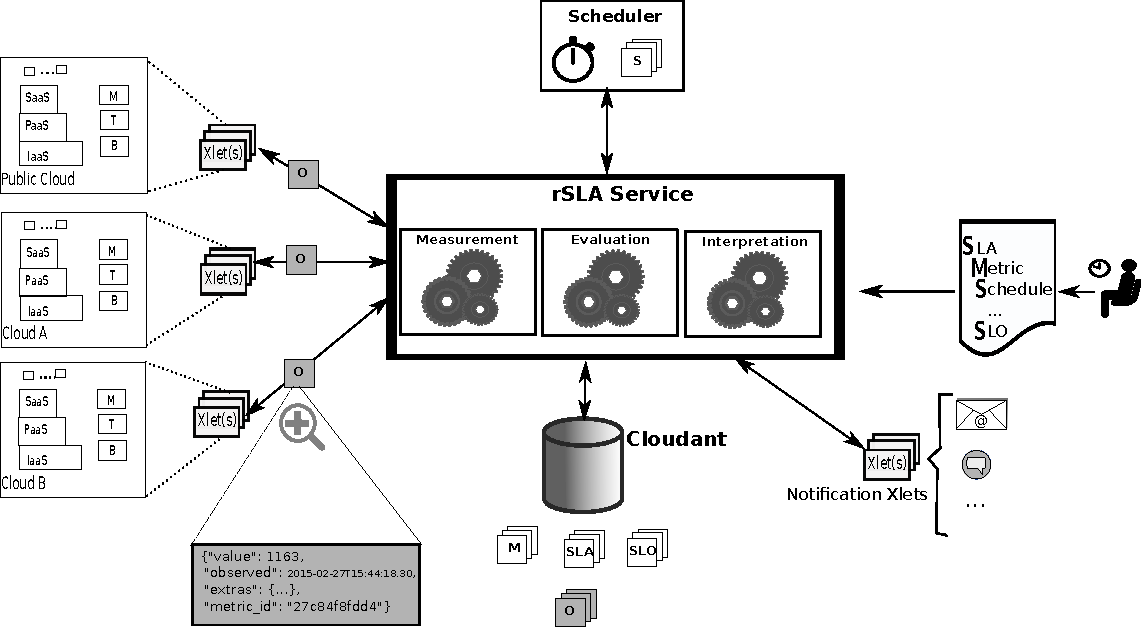
\includegraphics[width=\textwidth]{pics/runtime.pdf}
\caption{\label{fig:runtime} rSLA runtime}
\end{figure}


\subsection{Ameriprise pilot}

Currently, the rSLA service supports the management of cloud services that are leased by an existing customer. In one agreement, the IBM customer migrated a workload from a customer-owned, on-premise data center environment to the IBM cloud.  Along with the move, the customer required the monitoring of seven custom SLAs that had never been offered previously by the service provider in the cloud.

Each of the seven running SLAs consist of one base metric and one service level objective. The rSLA service that is running on the Bluemix platform, is aware of these seven agreements' context as such information is parsed by the rSLA engine to activate and initiate the measurement of involved base metrics. The rSLA service monitors, measures, evaluates and reports the service level status of the seven involved SLOs on a daily basis to the customer. 

%can we add a graph showing statistics on the rSLA service usage/performance since we started the ameriprise pilot? Bluemix?
%or from cloudant?



\subsection{rSLA service}
rSLA Service is a Sinatra application deployed on Bluemix PaaS. It offers different REST interfaces that allow the management of the life cycle of an SLA described using our DSL.
At the reception of a new SLA, rSLA Service interprets the file and creates ruby objects based on the DSL. The new objects are persisted in Cloudant using CouchRest Model.
On the activation of an SLA, rSLA Service orchestrates all the needed operations to activate and manage the SLA life cycle. It starts by scheduling data collection for base 
metrics. As shown in Figure~\ref{fig:runtime}, based on the defined schedules, the scheduler triggers the needed rSLA Service interfaces. This latter will then invoke the 
Monitoring Xlets to collect new observations for the related base metrics. Afterwards, the observations are persisted in Cloudant. Similarly, on the schedule of an SLO, the 
Scheduler triggers a rSLA Service interface for SLO evaluation. rSLA will then evaluate the data related to the specific SLO. This evaluation implies 
eventually the usage of map-reduce functions offered by Cloudant. We made this decision in order to delegate all the possible parallel processings to Cloudant and benefit from its 
efficiency. Afterwards, rSLA Service generates JSON notifications representing the results of the evaluation. These notifications are sent to the Notification Xlet for 
formatting and reporting to the client.   
\subsection{rSLA Xlets}
During its life-cycle, rSLA Service requires different services to ensure the management of SLAs. These services are eventually offered as services through Bluemix PaaS. At the 
time being, rSLA uses one offered service for persistence and a list of services for monitoring and reporting. These latter, are provided as Xlets. An Xlet is a light weight 
application offered as a service through Bluemix PaaS. This application is designed to facilitate the integration of different offered services spanning over the different layers 
of the Cloud by providing a generic REST API. An Xlet is customized according to its role in the overall system. As shown in Figure~\ref{fig:xlet}, each Xlet provides three 
interfaces:
\begin{itemize}
 \item \emph{CFBrokerInterface}: Since the Xlets are provided as services by Bluemix PaaS, they need to offer this generic interface that describes exactly how to provision the 
service, how to unprovision it, how to bind the service to a given application and how to unbind it. 
\item  \emph{ConfigurationInterface}: In order to ensure multi-tenancy and customization of an Xlet, it should offer an interface to configure its tenancy. This interface could 
offer other functionalities of customization. It allows in some cases to configure the access credentials for Cloud resources.
\item  \emph{RuntimeInterface}: This interface describes the main business of the Xlet. It describes the specific functionalities to be offered by the application instance (e.g., 
monitoring services, reporting services). 
\end{itemize}
\begin{figure}[H]
\centering
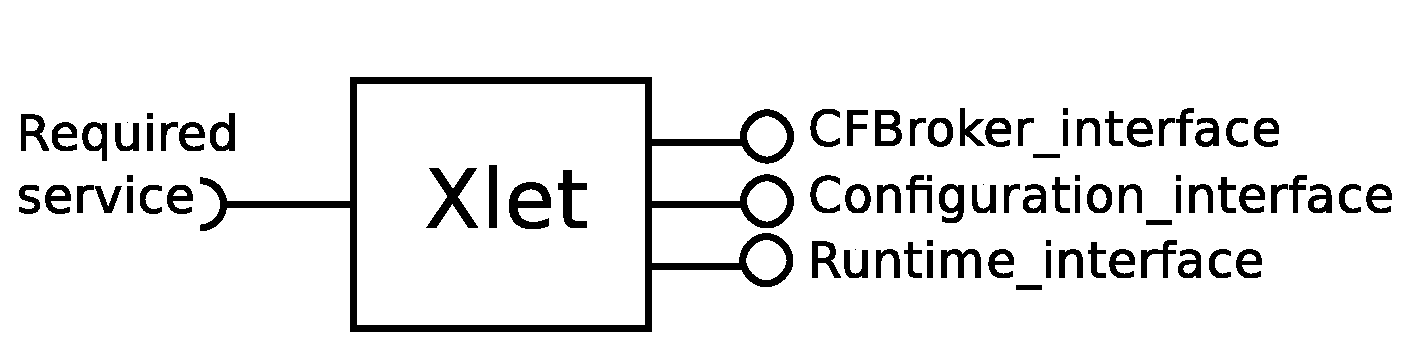
\includegraphics[width=0.6\textwidth]{pics/Xlet}
\caption{\label{fig:xlet} Xlet generic design}
\end{figure}

All Xlets respect the same architecture but differs in their implementations from a use case to another. In our current work we defined different monitoring and reporting Xlets. 
Monitoring Xlets are in-line with the DMTF standard. They allow collecting monitoring data for a specific type of resources with different granularities. For example, 
Figure~\ref{fig:slxlet} shows a SoftLayer specific Xlet. SLXlet allow to get monitoring data of SoftLayer provisioned servers for a given account. The account credentials are 
passed to the Xlet in the configuration phase through the Configuration interface. Afterwards, the Runtime interface of the Xlet could be used to get the list of servers, the list 
of metrics for a given server or, the value for a given metric for a specific server.

\begin{figure}[H]
\centering
\hspace{1.5cm}
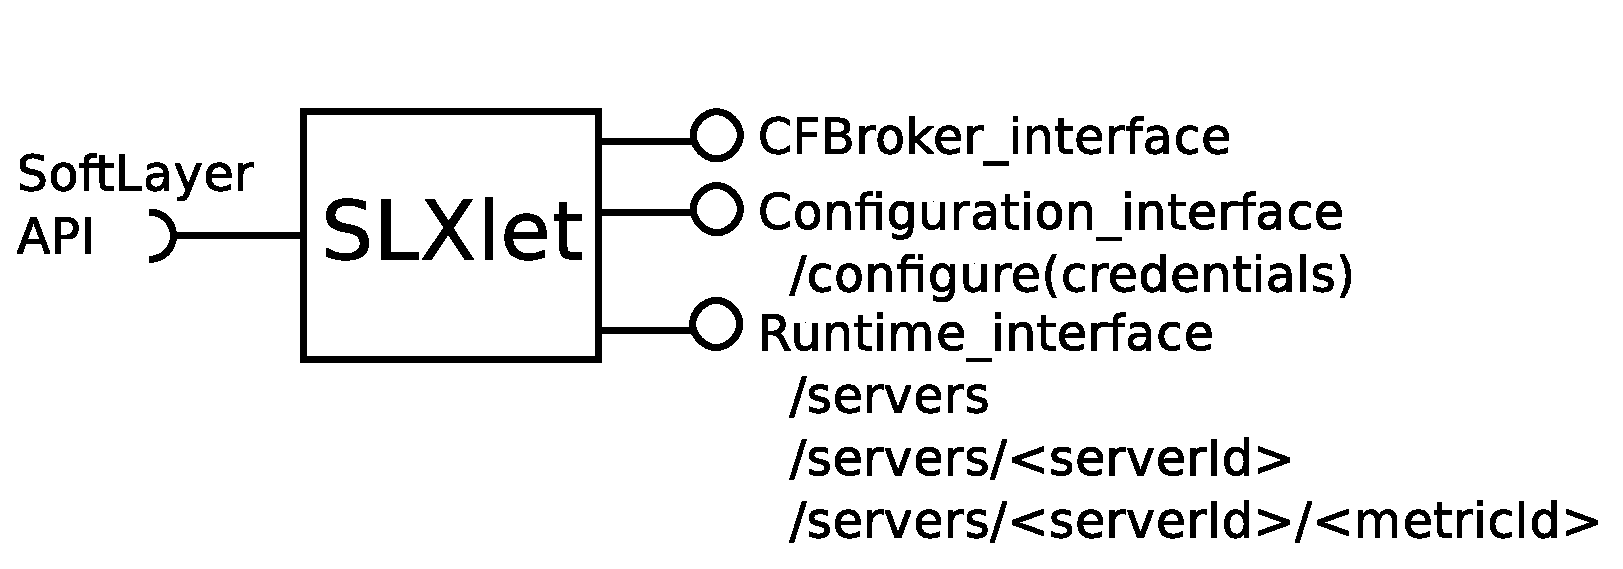
\includegraphics[width=0.7\textwidth]{pics/SLXlet}
\caption{\label{fig:slxlet} SoftLayer Xlet design}
\end{figure}

Using Xlets within Bluemix PaaS has been very helpful. The advantageous characteristics of using Xlets in this environment are the following:
\begin{itemize}
 \item Scalability: this characteristic is inherited from the scalability of Bluemix environment. Since the Xlet could be provisioned as an application or a service within 
Bluemix, it is easy to scale it horizontally to cope with the work load by adding or removing new instances,
\item Reusability: all Xlets have a common and generic core code that allow the easy reusability with minor modifications for specific use case, 
\item Manageability: managing Xlets is handled to Bluemix, the management here includes provisioning, deprovisioning, binding and unbinding Xlets to other applications,
\item Flexibility: Xlets could be integrated easily using Bluemix services, they could be provisioned using different plans (e.g., shared or dedicated). 
\end{itemize}
%
\section{rSLA implementation}\label{runtime} \todomohamed{rSLA implementation}

The rSLA is implemented as a DSL for cloud SLAs. The rSLA programming library, currently, provides support for the following SLA management operations that take place while a provisioned service is running:
\begin{enumerate}
\item SLA creation and activation.
\item monitoring and measurement of service metrics as specified by the SLA context.
\item storage and processing of observed service metric values and of SLO evaluation results. 
\item scheduling of rSLA objects.
\item service level evaluation.
\item notification events: reports.
\end{enumerate}
The next paragraphs highlight rSLA implementation aspects for all supported operations.

\subsection{SLA creation and activation}

As discussed in Chapter \ref{dsl}, rSLA editing takes place using ruby programming blocks. The rSLA language takes advantage of this Ruby coding feature and exposes rSLA objects through multi-lined do..end coding blocks. When an rSLA runtime engine reads a new rSLA block, it generates a new rSLA object that belongs to the block related class. The attributes and function behavior of the generated object are mapped from the ruby block context. 

Listing \ref{basescript} describes an rSLA script for the creation of an SLA and of a base metric. The script can run in an rSLA service runtime environment to generate the two respective objects and to activate a schedule for the value measurement of the base metric.

\begin{minipage}{0.9\textwidth}
\begin{lstlisting}[language=Ruby, basicstyle=\small\normalfont\sffamily, breaklines=true,  captionpos=b, mathescape=true, caption=rSLA SLA (lines 1-4) and basemetric (lines 6-19) creation script, label=basescript, numbers=left, numbersep=5pt, numberstyle=\tiny] 
sla do
  tenant "Demo"
  provider "IBM"
end  

basemetric do
    name "bareMetalProvisioning"
    unit "provisioningtime"
    measurementdirective do
    	entity "baremetal"
    	type "jsonArray"
    	source "http://provisioningxlet.stage1.mybluemix.net/server/baremetal/provisioningtime" 
  	end
  schedule do    
  	frequency "1"
    unit "m"
    method "every"
  end
end
\end{lstlisting}
\end{minipage} 

The block for the creation of the SLA object simply describes two strings that designate the names of the SLA tenant and provider. The rSLA engine reads such strings as the attribute values of the newly created SLA object. Similarly, the rSLA interpreter reads the base metric block and create a new base metric object that inherits the attributes of the rSLA BaseMetric class. 

In the base metric block, a DSL user can define BaseMetric object attributes like the base metric name and measurement unit. Additionally, a DSL user can specify directives for the measurement of the created metric. A measurement directive represents a concept that is inherited from the WSLA specification \cite{wsla}. 

The rSLA DSL exposes a measurement directive as a block of statements that a DSL user can specify. Such statements describe the configuration of a measurement directive object that guides the value measurement of the parent base metric. A measurement directive indicates the result type that is expected from a base metric measurement.

In the measurement directive block, the term entity is used for the representation of restful \footnote{ReST: \url{http://en.wikipedia.org/wiki/Representational_state_transfer}} endpoints. Such may have a URL\footnote{Unique Resource Locator: \url{http://en.wikipedia.org/wiki/Uniform_resource_locator}} form: \url{http://provisioningxlet.stage1.mybluemix.net/server/baremetal/provisioningtime}. A measurement directive object uses an attribute named $source$ to denote the restful endpoint for fetching the relevant base metric value. The rSLA MeasurementDirective class provides an example on how to define measurement directive objects for rSLA base metrics. Such example, like the illustrated block of Listing \ref{basescript} can be extended accordingly. 

Last but not least, a DSL user can specify the details of a schedule for the measurement of the base metric. The schedule block details are explained in Section \ref{schedule}.

\subsection{monitoring and measurement}
Any SLA management framework for cloud services needs a tool for monitoring and measuring service metric values. In a cloud runtime environment, an rSLA service currently uses Java Xlets \cite{xlets} to handle the monitoring of base betric values. Chapter \ref{deployment} describes in detail the configuration and functionality of Xlets with the deployment of rSLA as a compliance service in a cloud environment.

In an rSLA service, monitoring and measurement operations are controlled by one or more schedules. Every base metric follows its own schedule. Measured metric values are collected to a backend database for further processing. 
\subsection{storage and processing}
Currently, rSLA is deployed as a service on the IBM Bluemix platform \cite{bluemix} and is configured to use a Cloudant \cite{cloudant} document database. The values of base metrics are preserved as observation documents with a timestamp on the measurement time and the associated base metric id. Cloudant uses map and reduce statements to collect and to efficiently process data values. 

Observed values of base metrics are stored, while a provisioned service is running. These data values are required for the computation of composite metric values that are used by the service level evaluation. 

rSLA uses CouchRest \cite{couchrest} to access Cloudant through HTTP requests and CouchRest model to map rSLA object properties in the database. Associations between rSLA objects are, at the present time, described through the rSLA Cloudant data schema. Figure \ref{schema} illustrates  associations between rSLA objects in a Cloudant database.

Base, composite metrics as well as SLOs are associated with an SLA instance by a \textit{belongs to} relationship. Similarly, a set of observations \textit{belongs to} a base metric and a set of evaluation and notification data to an SLO. 

The \textit{belongs to} feature is defined in the CouchRest model as a property for the association of documents. It resembles a \textit{has-a} composition relationship \footnote{\url{http://en.wikipedia.org/wiki/Has-a}} where a constituent object belongs to or is part of the definition of another object.

\begin{figure}
\centering
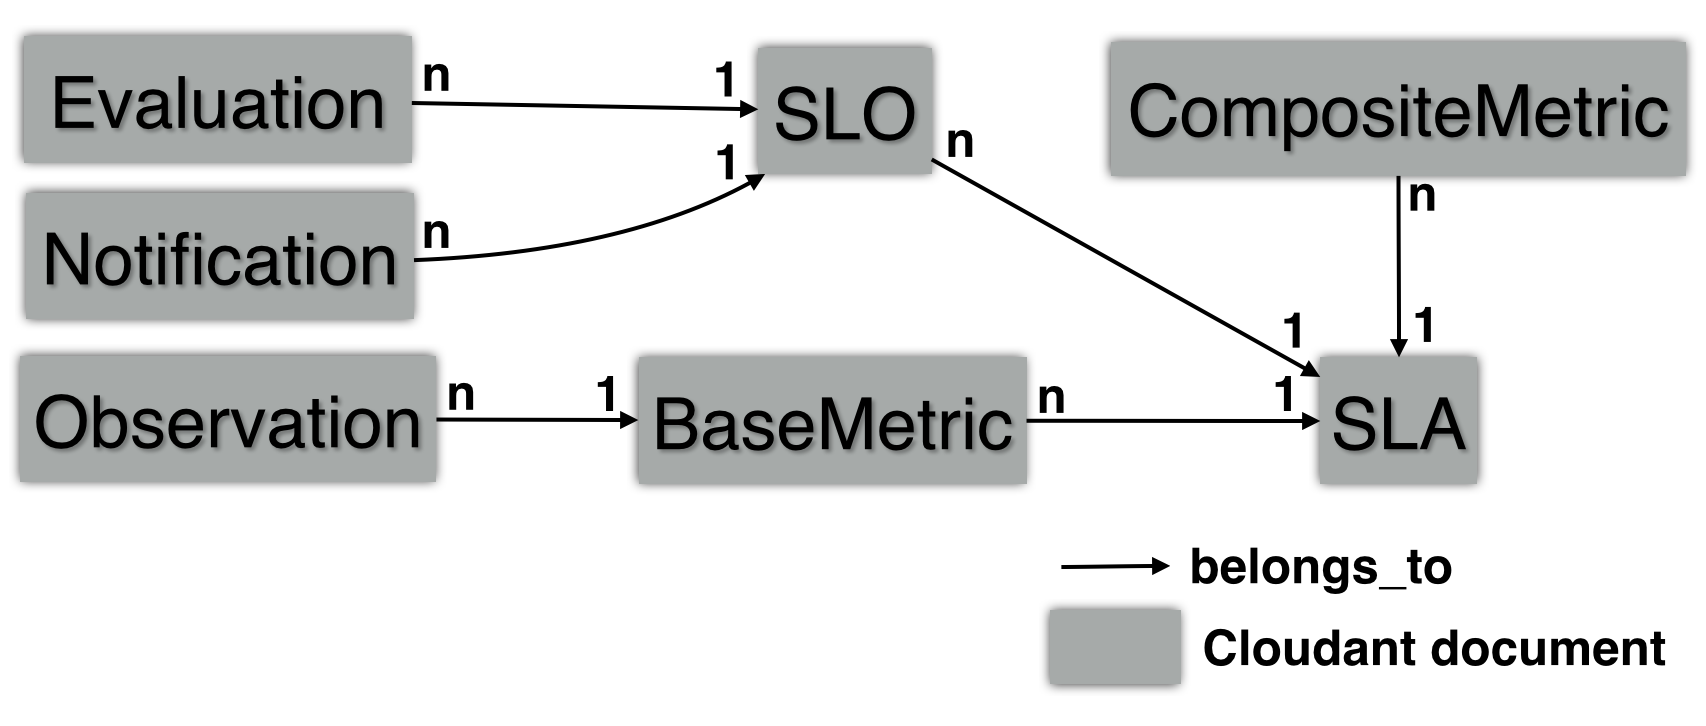
\includegraphics[width=0.8\textwidth]{pics/schema}
\caption{\label{schema} rSLA Cloudant object associations}
\end{figure}

At the current development state of the rSLA language, processing of service metric values may refer to compositions of base and composite metric value sets for the creation of composite metrics or of rSLA expression objects. In rSLA language, the definition of composite metrics represents the outcome from combining a set of base and/or composite metrics. The value computation of such metrics represents a computation that comprises values of other metrics. 

As discussed in Section \ref{dsl}, expressions in rSLA denote free form statements that may take a conditional form or that may define data value computations. The computation for a composite metric value exemplifies an expression in rSLA. Composite metric values are used for the SLO evaluation. rSLA expressions that are defined as either SLO precondition or objectives may refer to composite metric values.

Last but not least, the rSLA language library contains also a time series class that can be used for the application of statistical functions on time-series data sets. 

\subsection{scheduling}\label{schedule}
The rSLA BaseMetric class provides methods for configuring a base metric object with one or more schedules. In an rSLA runtime environment, a scheduler orchestrates the activation, monitoring and processing of rSLA objects.

When the rSLA engine reads an rSLA script file and generates a new SLA object, the SLA object is inactive. The inactive state indicates that the SLA object is not associated with any service metrics that require measurement. It also designates that a scheduler is unaware of the SLA object creation and thus unaware of all rSLA objects that are defined in the new rSLA tree.

On SLA activation, the rSLA engine collects all base metrics that are included under the new SLA and activates them by sending their schedule and id to a scheduler. The scheduler uses the base metric input to create scheduling events for each of the base metrics. 

In rSLA, composite metrics do not include a schedule because the computation of their values depends from SLO evaluation events. The SLO definition specifies a schedule for the evaluation of precondition and objective expressions. Moreover, a scheduler orchestrates notification processes that send evaluation reports on scheduled intervals.

The orchestration of scheduling events represents a topic of on-going work. Currently, rSLA uses the rufus-scheduler that is an in-memory Ruby scheduler. 

\subsection{service level evaluation}

In an rSLA runtime environment, service level evaluation takes place at scheduled intervals. The frequency of service level evaluation is determined by the schedule attributes in the SLO definition. As discussed in Section \ref{dsl}, the definition of a service level objective encloses the description of a precondition and of an objective expressions. These two expressions that follow sequential logic, define the evaluation conditions that designate if the state of an SLO is healthy or not.

We can symbolically define such expressions as the union of composite metric values, hence 


\subsection{notification reports}
can also be alerts
rSLA needs a source for monitoring data and a tool for reporting.
%
\section{Conclusions}
\todoall{conclusions, challenges and on-going work}

\bibliographystyle{splncs}

\bibliography{mainDoc}

%----------------------------------------------------------------------------------------


\end{document}
